\documentclass[11pt]{article}
\usepackage{laboratory}
\usepackage{tikz}
\usetikzlibrary{arrows.meta, positioning}

% A count averaged over three runs, with the lowest and highest run beside it.
\newcommand{\runs}[3]{\num{#1} & {\footnotesize\color{black!60}(\numrange{#2}{#3})}}
\newcommand{\steady}[1]{\num{#1} &}

\title{Verified answers from component datasheets}
\author{Shlok Bhusal}
\date{November 2026}
\source{github.com/Protonicwave/\newline datasheet-question-answering-assistant}

\begin{document}

\maketitle

\begin{abstract}
A language model asked about a sensor datasheet can state a wrong value with nothing to show which value is wrong. This assistant answers from passages retrieved from six Bosch Sensortec datasheets and shows an answer only when code confirms that each quoted passage appears word for word on the cited page and that every number in the answer appears in a quote. A rejected answer is sent back to the model once with the reason. On 50 held-out questions, 40 of them answerable, the model alone answered 26.0 correctly per run and stated a wrong value for 4.3. With retrieval it answered 33.3 correctly, with one wrong answer in three runs, and that answer traces to a datasheet that gives two values for one quantity. The check alone withheld 7.3 correct answers per run; with one revision the assistant answered 32.7 correctly with 4.0 answerable questions declined, against 3.3 for unchecked retrieval. The check does not make answers more accurate. It guarantees that every number shown can be found in a passage on the page cited.
\end{abstract}

\section{Introduction}
\label{sec:introduction}

A model answering datasheet questions from memory states wrong values; this assistant shows a value only when code finds it in a passage quoted from the cited page.

\section{System}
\label{sec:system}

Each question passes through retrieval, an answer with citations, the check and at most one revision, and ends in one of three outcomes. \Cref{fig:pipeline} shows the path; this section takes each step in turn.

\begin{figure}[tbp]
  \centering
  \begin{tikzpicture}[
      font=\sffamily\small,
      node distance=10mm and 8mm,
      box/.style={draw=black!70, rounded corners=2pt, align=center, inner sep=4pt, minimum height=11mm},
      check/.style={box, draw=prussian, very thick},
      outcome/.style={align=center, inner sep=2pt, text=prussian},
      flow/.style={-{Stealth[length=2mm]}, black!70},
      label/.style={font=\sffamily\footnotesize},
    ]
    \node[box] (question) {Question};
    \node[box, right=of question] (search) {BM25 search\\8 excerpts};
    \node[box, right=of search] (answer) {Model answer\\with citations};
    \node[check, right=of answer] (check) {Check\\quote and numbers};
    \node[outcome, right=of check] (shown) {Verified answer\\shown};
    \node[box, below=of check] (revise) {One revision\\with the reason};
    \node[outcome, right=of revise] (withheld) {No verified\\answer};
    \node[outcome, below=of answer] (none) {The datasheet\\does not say};

    \draw[flow] (question) -- (search);
    \draw[flow] (search) -- (answer);
    \draw[flow] (answer) -- (check);
    \draw[flow] (check) -- node[label, above] {pass} (shown);
    \draw[flow] ([xshift=-5mm]check.south) -- node[label, left] {fail} ([xshift=-5mm]revise.north);
    \draw[flow] ([xshift=5mm]revise.north) -- node[label, right] {recheck} ([xshift=5mm]check.south);
    \draw[flow] (revise) -- node[label, above] {fail} (withheld);
    \draw[flow] (answer) -- node[label, left] {unanswerable} (none);
  \end{tikzpicture}
  \caption{The path of one question. Only an answer that passes the check is shown. A rejected answer is sent back once with the reason it failed, and a revision that also fails is withheld.}
  \label{fig:pipeline}
\end{figure}

\subsection{Pages and text}

The datasheets are downloaded from Bosch Sensortec and checked against a SHA-256 hash recorded in the repository, so every run reads the same files; the PDFs themselves are not redistributed. The text of each page is extracted with pdfium. Table rows come out in reading order, one row to a line, but the column a value sat in is lost: a row of minimum, typical and maximum values reads \enquote{\texttt{1.8 2.8 µA}} with no sign of which column was empty. Figures and graphs carry no text layer and are invisible to the assistant.

One normaliser prepares text for both search and the check, so the two never disagree about what a page says. It applies Unicode compatibility folding, maps the Unicode minus sign and every dash to a hyphen, unifies the two micro signs, removes a hyphen between two letters, and collapses runs of white space. The hyphen rule exists because pdfium marks a line-break hyphen with one code point whether the word was split (\enquote{consist-ing}) or genuinely hyphenated (\enquote{low-power}); removing every hyphen between letters on both sides of the comparison makes both spellings match.

\subsection{Retrieval}

Each page is cut into chunks of whole lines, merged up to about 300 words and never spanning two pages, and each chunk keeps its datasheet and page. Search ranks chunks with BM25~\cite{robertson2009}, with $k_1 = 1.2$ and $b = 0.75$, and passes the top eight, about 2,400 words, to the model. BM25 was chosen over embeddings because datasheet questions turn on exact terms such as register names, and because it is deterministic. When a question names a part, only that part's datasheet is searched. Without this rule a BMP390 question ranked BMA456 and BMI270 pages first: every page header repeats the part number, so as a search term it barely separates one datasheet from another. A question that shares no term with any chunk is declared unanswerable without a model call.

\subsection{Answer}

The model, \texttt{claude-sonnet-5-5}, receives the excerpts, each marked with its datasheet and page, and returns a structured reply: whether the excerpts answer the question, a short answer, and one to three citations, each naming a datasheet and page and quoting a passage of at least four words. The prompt asks for numbers written as the datasheet writes them, no unit conversions, and no number repeated from the question unless a quote contains it. A request the API refuses or truncates, a failed request, or a reply that does not match the schema is recorded as an error, never as a sign that the datasheet does not say.

\subsection{The check}

The check is a pure function of the answer and the page texts. An answer passes only if it cites at least one passage; every citation names a datasheet and page that exist; every quote is at least four words long and appears, after normalisation, on the page it cites; and every number in the answer appears in at least one of its quotes. The four-word minimum stops a quote such as \enquote{\qty{3.6}{\volt}}, which appears on many pages, from passing as evidence. The numbers are pooled across citations because one answer may combine values from up to three passages.

Numbers are extracted as signed decimals, scientific notation and hexadecimal (\texttt{0x76}). A digit attached to letters, as in \texttt{BME280} or \texttt{I2C}, is not a number, and an \texttt{x} between digits separates two values, so \texttt{2.5x3.0} yields 2.5 and 3.0. Decimals compare by value with their sign, so 3.30 matches 3.3 but $-40$ does not match 40; hexadecimal compares as text, ignoring case.

\subsection{Revision and outcomes}

A rejected answer is sent back to the model in the same conversation, followed by the reason it failed, for example \enquote{answer states 0, 2, which no quote contains}. The model is asked to fix the cause, either by quoting a passage that holds the number or by leaving out a number the question did not ask for, and is told not to drop the value the question asks for. One revision is allowed. The revision faces the same check, so it can move an answer from withheld to shown only by passing.

Each question ends in one of three outcomes. A verified answer is shown with its citations. \enquote{No verified answer} means every draft failed the check: the datasheet may still state the value, and the reason is shown. \enquote{The datasheet does not say} means the model found no passage that answers. A web page shows each verified answer beside the rendered datasheet page with the quoted passage highlighted, and marks a number's place on the page when the reader points at it in the answer.

\section{Evaluation}
\label{sec:evaluation}

Four arms answer the same questions on six datasheets, three runs each, and code scores every answer against expected numbers and keywords.

\section{Results}
\label{sec:results}

\Cref{tab:held-out} gives the held-out counts for every arm and \cref{fig:results} plots the three that separate them.

\begin{table}[tbp]
  \centering
  \caption{Held-out set: 50 questions, 40 answerable, three runs per arm. Each count is the mean over the runs, with the lowest and highest run in brackets where they differ. No arm returned an API error.}
  \label{tab:held-out}
  \begin{tabular}{
    l
    S[table-format=2.1] l
    S[table-format=1.1] l
    S[table-format=2.1] l
    S[table-format=2.1] l
    S[table-format=1.1] l
  }
    \toprule
    \head{Arm} & \multicolumn{2}{l}{\head{Correct}} & \multicolumn{2}{l}{\head{Wrong}} & \multicolumn{2}{l}{\head{Correct refusal}} & \multicolumn{2}{l}{\head{False refusal}} & \multicolumn{2}{l}{\head{Unplaced}} \\
    \midrule
    A: model alone & \steady{26.0} & \runs{4.3}{3}{7} & \runs{9.7}{9}{10} & \runs{9.7}{8}{11} & \runs{0.3}{0}{1} \\
    B: model with search & \runs{33.3}{33}{34} & \runs{0.3}{0}{1} & \steady{10.0} & \runs{3.3}{3}{4} & \steady{3.0} \\
    C: search with check & \runs{26.0}{25}{27} & \runs{0.3}{0}{1} & \steady{10.0} & \runs{10.7}{9}{12} & \steady{3.0} \\
    D: search, check and retry & \runs{32.7}{32}{34} & \runs{0.3}{0}{1} & \steady{10.0} & \runs{4.0}{3}{5} & \steady{3.0} \\
    \bottomrule
  \end{tabular}
\end{table}

\begin{figure}[tbp]
  \centering
  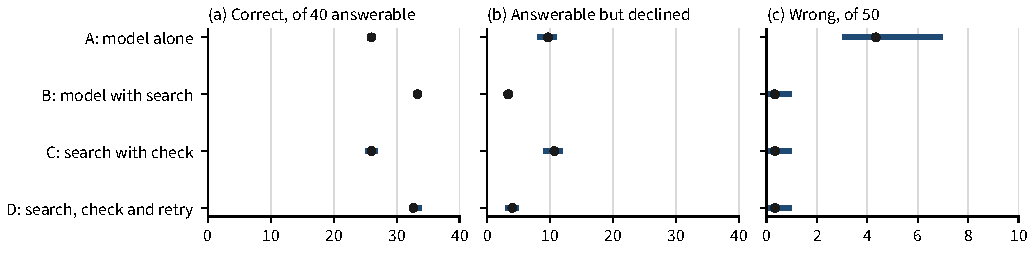
\includegraphics[width=\linewidth]{figures/results}
  \caption{Held-out results per arm. Each dot is the mean of three runs and the bar spans the lowest to the highest run. Panel (c) counts all 50 questions, since answering an unanswerable question is also wrong.}
  \label{fig:results}
\end{figure}

The model alone answered 26.0 of the 40 answerable questions correctly and gave a wrong answer to 4.3 questions per run, between 3 and 7. Its 13 wrong answers over three runs fell on seven questions. Two were wrong in every run, the BMA456 \texttt{INIT\_CTRL} reset value and the BMA456 sensor time increment discussed below, and two in two runs, the BMA456 filter bandwidth at an output data rate of \qty{100}{\hertz} and the BHI360 gyroscope sensitivity. Eight of the 13 answers said they came from memory or were uncertain; all 13 stated a value. One of the 13 answered an unanswerable question, and three are the sensor time answers, where the fault lies in the question; without those three, A gave 3.3 wrong answers per run.

With search, the model answered 33.3 correctly, refused all ten unanswerable questions in every run and gave one wrong answer in three runs. Every correct answer cited a page the question lists as stating the value. The three unplaced answers per run are correct when read by hand: each writes the unit against the number, as in \enquote{1.25ms}, \enquote{12.5MHz} and \enquote{0.4mm}, and the scorer's whole-word match does not find \enquote{ms} in \enquote{1.25ms}. The same three answers are unplaced in arms C and D.

The check alone withheld 22 of B's answers over the three runs, 7.3 per run, and every one was to an answerable question. Twelve quoted fewer than four words. Ten stated a number that no quote contained: in six the number was part of register notation, such as \enquote{bits 3..1} or \texttt{int\_latch='0'}, and in the rest an operating condition, a table number or a page number mentioned in passing. C's correct count fell to 26.0 and its false refusals rose from B's 3.3 to 10.7. The check removed none of B's wrong answers: the one wrong answer passed it.

With one revision, D revised all 22 withheld answers and showed 20, each scored correct. The two it still withheld were the same question in two runs: the answer repeated the field name \texttt{t\_sb[2:0]} from the question, and the check read 2 and 0 as numbers no quote contained. D answered 32.7 correctly with 4.0 false refusals: two answers in three runs behind B, 0.7 per run on each count.

The single wrong answer of arms B, C and D is the same answer in run 2 to the question of how often the BMA456 \texttt{SENSORTIME\_0} register increments. Page 16 of the datasheet says the register increments every \qty{39.25}{\micro\second}, and the question expects that value; pages 21 and 51 give \qty{39.0625}{\micro\second}~\cite{bma456}. In runs 1 and 3 the answer quoted both pages and stated both values, which the scorer accepts. In run 2 it quoted only pages 21 and 51 and gave \qty{39.0625}{\micro\second}, a value the datasheet does state. The model alone gave \qty{39.0625}{\micro\second} in all three runs. The datasheet contradicts itself, so these answers are scored wrong as committed but the fault lies in the question.

\Cref{tab:development} gives the development figures. They follow the same pattern with larger gaps: the check alone cost B 24.3 correct answers per run, and all 73 withheld answers passed the check after one revision, so a second revision was never requested. D's 0.3 shortfall against B is one revised answer, \enquote{1ms}, that is correct by hand but unplaced by the scorer. The limit was then lowered from two revisions to one, which leaves these figures unchanged and cuts the worst case from three requests per question to two.

\begin{table}[tbp]
  \centering
  \caption{Development set: 100 questions, 80 answerable, three runs per arm. These questions were read while the revision step was designed, so the figures show why it exists and are not the result. No arm returned an API error.}
  \label{tab:development}
  \begin{tabular}{
    l
    S[table-format=2.1] l
    S[table-format=2.1] l
    S[table-format=2.1] l
    S[table-format=2.1] l
    S[table-format=1.1] l
  }
    \toprule
    \head{Arm} & \multicolumn{2}{l}{\head{Correct}} & \multicolumn{2}{l}{\head{Wrong}} & \multicolumn{2}{l}{\head{Correct refusal}} & \multicolumn{2}{l}{\head{False refusal}} & \multicolumn{2}{l}{\head{Unplaced}} \\
    \midrule
    A: model alone & \runs{59.7}{58}{62} & \runs{11.0}{9}{13} & \runs{14.3}{13}{15} & \runs{15.0}{12}{17} & \steady{0.0} \\
    B: model with search & \steady{77.0} & \steady{0.0} & \steady{20.0} & \steady{3.0} & \steady{0.0} \\
    C: search with check & \runs{52.7}{52}{54} & \steady{0.0} & \steady{20.0} & \runs{27.3}{26}{28} & \steady{0.0} \\
    D: search, check and retry & \runs{76.7}{76}{77} & \steady{0.0} & \steady{20.0} & \steady{3.0} & \runs{0.3}{0}{1} \\
    \bottomrule
  \end{tabular}
\end{table}

\section{Discussion and limits}
\label{sec:discussion}

Search, not the check, removed the wrong answers. The model alone gave a wrong value for 4.3 held-out questions per run; with eight retrieved excerpts it gave one wrong answer in three runs, and that answer quoted a real passage, so the check passed it. On these questions the check did not make the shown answers more accurate.

What the check bought is a property of every answer shown: each number in it appears in a passage quoted word for word from the page it cites. A reader who doubts a value opens one page, finds a highlighted passage and confirms the number there, rather than searching the datasheet. Without the check, arm B's answers carry the same citations, but nothing confirms that the quote is on the page or that the number is in the quote. On this set B's citations happened to hold up; the check is what makes that true of every answer rather than of those examined.

The check alone paid for this property with recall: it withheld 7.3 of B's 33.3 correct held-out answers per run. Its rejections were mostly the model's own habits rather than unsupported claims. A three-word quote such as \enquote{\enquote{110}: 10 ms} is the right evidence and simply too short for the rule; \enquote{bits 3..1} is register notation the model wrote in its own words. Because these rejections are systematic, sending the reason back works: one revision recovered 20 of the 22 withheld answers and brought arm D to within 0.6 correct answers and 0.7 false refusals of B. The two answers it could not recover came from one case the check gets wrong. A field name taken from the question, \texttt{t\_sb[2:0]}, contains digits, and the check counts them as numbers the quote must contain. Exempting text copied from the question would fix this case, but it would also let an answer repeat a wrong value that the question itself contained.

\subsection{What the check does not catch}

The check confirms that a number is in a quote and the quote is on a page. It does not confirm that the quote answers the question. An answer can quote the wrong row, the wrong condition or the wrong column of a table and pass, and the BMA456 sensor time question shows that a datasheet can state two values for one quantity. A revision can also pass by dropping context: in the development run, one revision dropped the $\pm 8\,g$ range from an answer about the accelerometer's reset range, and it was still scored correct. The revision prompt forbids dropping the value the question asks for, but nothing in code enforces it, and a revision could in principle swap the requested value for another number from the same quote. The scorer would count a swapped value as wrong, but it cannot see dropped context, and the assistant prevents neither.

\subsection{What the assistant cannot read}

The assistant reads only the text layer. Graphs, timing diagrams and package drawings are invisible to it, and formulas extract as garbled text. In tables the column a value sat in is lost, so a row of minimum, typical and maximum values cannot tell the model which is which; two of the withheld held-out answers said as much. The number extractor reads \enquote{10,000} as 10 and 0, so a value written with a thousands separator can be neither verified nor scored, and one held-out candidate was dropped for that reason. The check compares numbers as written, so an answer converted from \qty{1}{\milli\ampere} to \qty{1000}{\micro\ampere} is withheld, and the prompt asks the model not to convert. Decimal commas and scanned datasheets without a text layer are not handled.

\subsection{How far the result reaches}

The held-out result rests on 50 questions, 40 of them answerable, on six datasheets from one manufacturer, answered by one model. The questions are on the same datasheets as the development set, so they test the system on new questions, not on new documents. The held-out set was drafted and checked by Claude, and Claude also answers the questions; a person checking each question against the PDF, as was done for the development set, would make the set independent of the model it measures. Three runs show how much the counts move between runs, at most four questions for any arm and category, but they are too few for an interval. The scorer undercounts correct answers when the unit is written against the number, which leaves three correct answers per run unplaced in arms B to D, and it marks a correct answer wrong when the question records only one of two values that the datasheet gives.

\section{Conclusion}
\label{sec:conclusion}

The check costs recall and buys a guarantee, and one revision with the rejection reason recovers most of the recall.


\bibliographystyle{apsrev4-2}
\bibliography{refs}

\appendix
\section{Reproducing the results}
\label{sec:reproduction}

The repository's README gives installation. A run needs the datasheets ingested and an Anthropic API key in the environment variable \texttt{ANTHROPIC\_API\_KEY}. One command then produces each run:

\begin{lstlisting}[language={}]
uv run datasheet-assistant ingest
uv run datasheet-assistant evaluate --questions eval/held_out.jsonl --runs 3
\end{lstlisting}

Each run writes a new directory under \texttt{eval/runs/} holding every answer with its citations and revisions (\texttt{answers.jsonl}), the score of each question per arm and run (\texttt{scores.csv}) and the counts per arm (\texttt{summary.csv}, \texttt{summary.md}). \Cref{tab:runs} lists the committed runs. A rerun makes new model requests, so its counts will differ from these within roughly the spread the tables show.

\begin{table}[htbp]
  \centering
  \caption{Committed evaluation runs. The held-out set was committed at \texttt{4b9dc7c} and run once at that commit.}
  \label{tab:runs}
  \begin{tabular}{llll}
    \toprule
    \head{Run directory} & \head{Question set} & \head{Arms} & \head{Results commit} \\
    \midrule
    \texttt{20261108T120946Z} & development & A to C & \texttt{be39273} \\
    \texttt{20261108T125938Z} & development & A to D, up to two revisions & \texttt{91bd5e1} \\
    \texttt{20261108T135144Z} & held-out & A to D, one revision & \texttt{164ba5b} \\
    \bottomrule
  \end{tabular}
\end{table}

The figure in \cref{sec:results} is drawn from the held-out \texttt{summary.csv} by \texttt{docs/report/figures/results.py}:

\begin{lstlisting}[language={}]
uv run --group docs python docs/report/figures/results.py
\end{lstlisting}


\end{document}
